\chapter{Introduction}
\label{ch:intro}
\epigraph{What we call the beginning is often the end. And to make an end is to make a beginning.}{\textsc{T.S. Eliot}}


This dissertation presents a general approach to improve visual egomotion estimation for mobile autonomous platforms.  In the broadest sense, \textit{egomotion estimation} refers to the process of computing the motion of a rigid body---relative to a fixed frame of reference---using measurements from sensors attached to the body (hence \textit{ego}motion\footnote{To the best of the author's knowledge, this term originates from experimental psychology \citep{warren1976perception}, and was also referred to as \textit{passive navigation} in the context of camera motion \citep{bruss_passive_1983}.}).  
\begin{remark}{Autonomy through history}
Mobile \textit{automata} have been a part of human culture since antiquity. In ancient India, the king Ajatashatru was said to use \textit{bhuta vahana yanta} (`spirit movement machines') to protect the relics of Gautama Buddha after his death in the fourth century BCE. According to Burmese legend, the bhuta vahana yanta of Ajatashatru were made with stolen secrets from a group of Greco-Roman `roboticists' named the \textit{yantakara}. The methods of the yantakara were closely guarded, and mechanical assassins were said to pursue those who attempted to disseminate them \citep{MayorGodsRobots2019}.

In the millennia since, mobile automata were relegated to isolated demonstrations (e.g., the programmable cart of Hero of Alexandria or the `autonomous' knight of Leonardo da Vinci) or to imagined forms in cautionary tales (e.g., Mary Shelley's \textit{Frankenstein}). Although the secrets of the yantakara may never be rediscovered, the ancient pursuit of helpful automata has found new life towards the turn of the twenty-first century and yielded machinery and algorithms that show great promise in aiding humanity.
\end{remark}
 
 \begin{wrapfigure}{r}{0.48\textwidth}
	\centering
	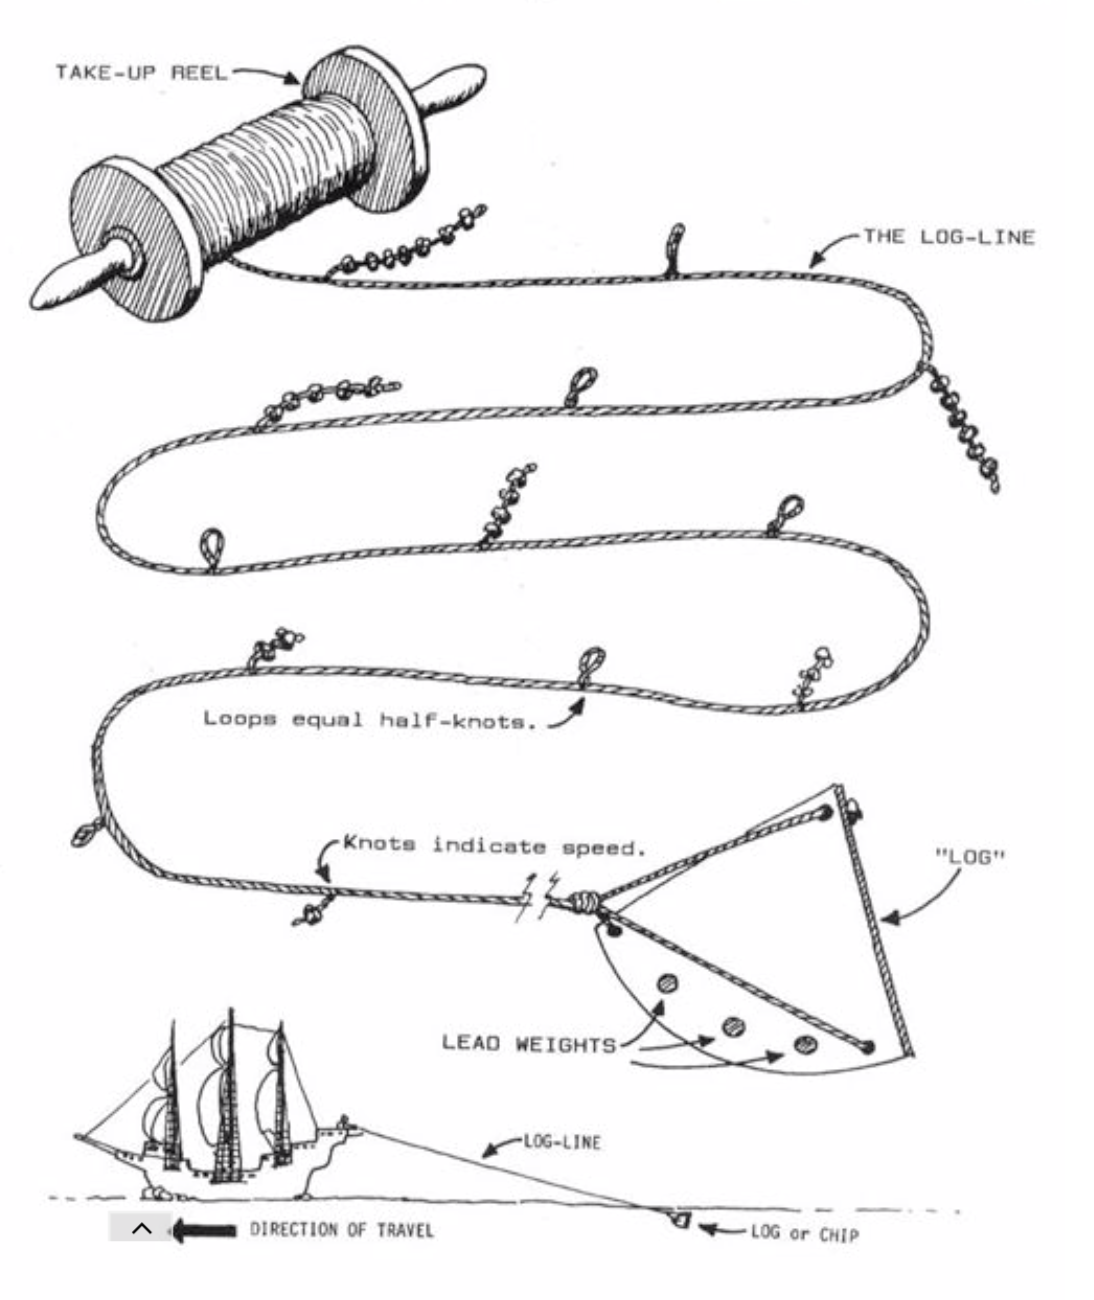
\includegraphics[width=0.48\textwidth]{introduction/chip_log}
	\caption{A \textit{chip log} is a historical tool used to measure ship speed. The \textit{log} or \textit{chip} was tossed into the water, and speed was measured by the amount of \textit{knots} that unravelled in a set time interval (\textit{credit: oceonmotion.org}).}
	\label{fig:intro_chip_log}
\end{wrapfigure}

 One way to estimate egomotion is to measure rates (e.g., linear or rotational velocities) and integrate them to compute changes in position and orientation. This method, referred to as \textit{dead reckoning}, was used by marine navigators of ancient times to determine the longitude of a ship at sea. Unlike latitude, which navigators could determine by measuring the altitude of the noon Sun, or the altitude of Polaris (the North Star) at night, longitude was not reliably computed from celestial measurements until the development of the marine chronometer in the 18th century \citep{Barfoot2017-ri}. As a result, early seafarers could only \textit{dead reckon} east-west motion by relying on estimates of local water currents, and by measuring the ship's magnetic heading and its speed relative to water (through a tool called a \textit{chip log}, \Cref{fig:intro_chip_log}). 

In a similar process, early aviators computed egomotion through magnetic heading, airspeed, and an estimate of prevailing winds. While even modern egomotion estimation methods exhibit unbounded error growth \citep{Olson2003-ax}, these early techniques were particularly inaccurate and required regular corrections through observations of known landmarks.\footnote{Perhaps the most famous example of dead-reckoning error was made by Christopher Columbus in 1492. He believed he had reached the \textit{Indies} (modern Indonesia) but had really arrived in the Bahamas.} In the mid twentieth century, the goals of inter-continental flight and space exploration necessitated the development of more accurate egomotion sensors (e.g., gimballed inertial platforms including accelerometers and gyroscopes) and an associated set of estimation techniques that could compute egomotion without human intervention (e.g., the Kalman filter \citep{Grewal2010-ts}).


By the late twentieth century, unmanned Lunar and Martian exploration motivated the development of a new approach to egomotion estimation. Although ground vehicles like extra-planetary rovers could infer egomotion through \textit{wheel odometry} (integrating wheel rates and using wheel orientation to drive a kinematic model), this approach was highly inaccurate on surfaces that induce wheel slip (e.g., the rock and sand covered surface of Mars, \Cref{fig:intro_endeavour_crater}). 

\begin{wrapfigure}{r}{0.45\textwidth}
	\centering
	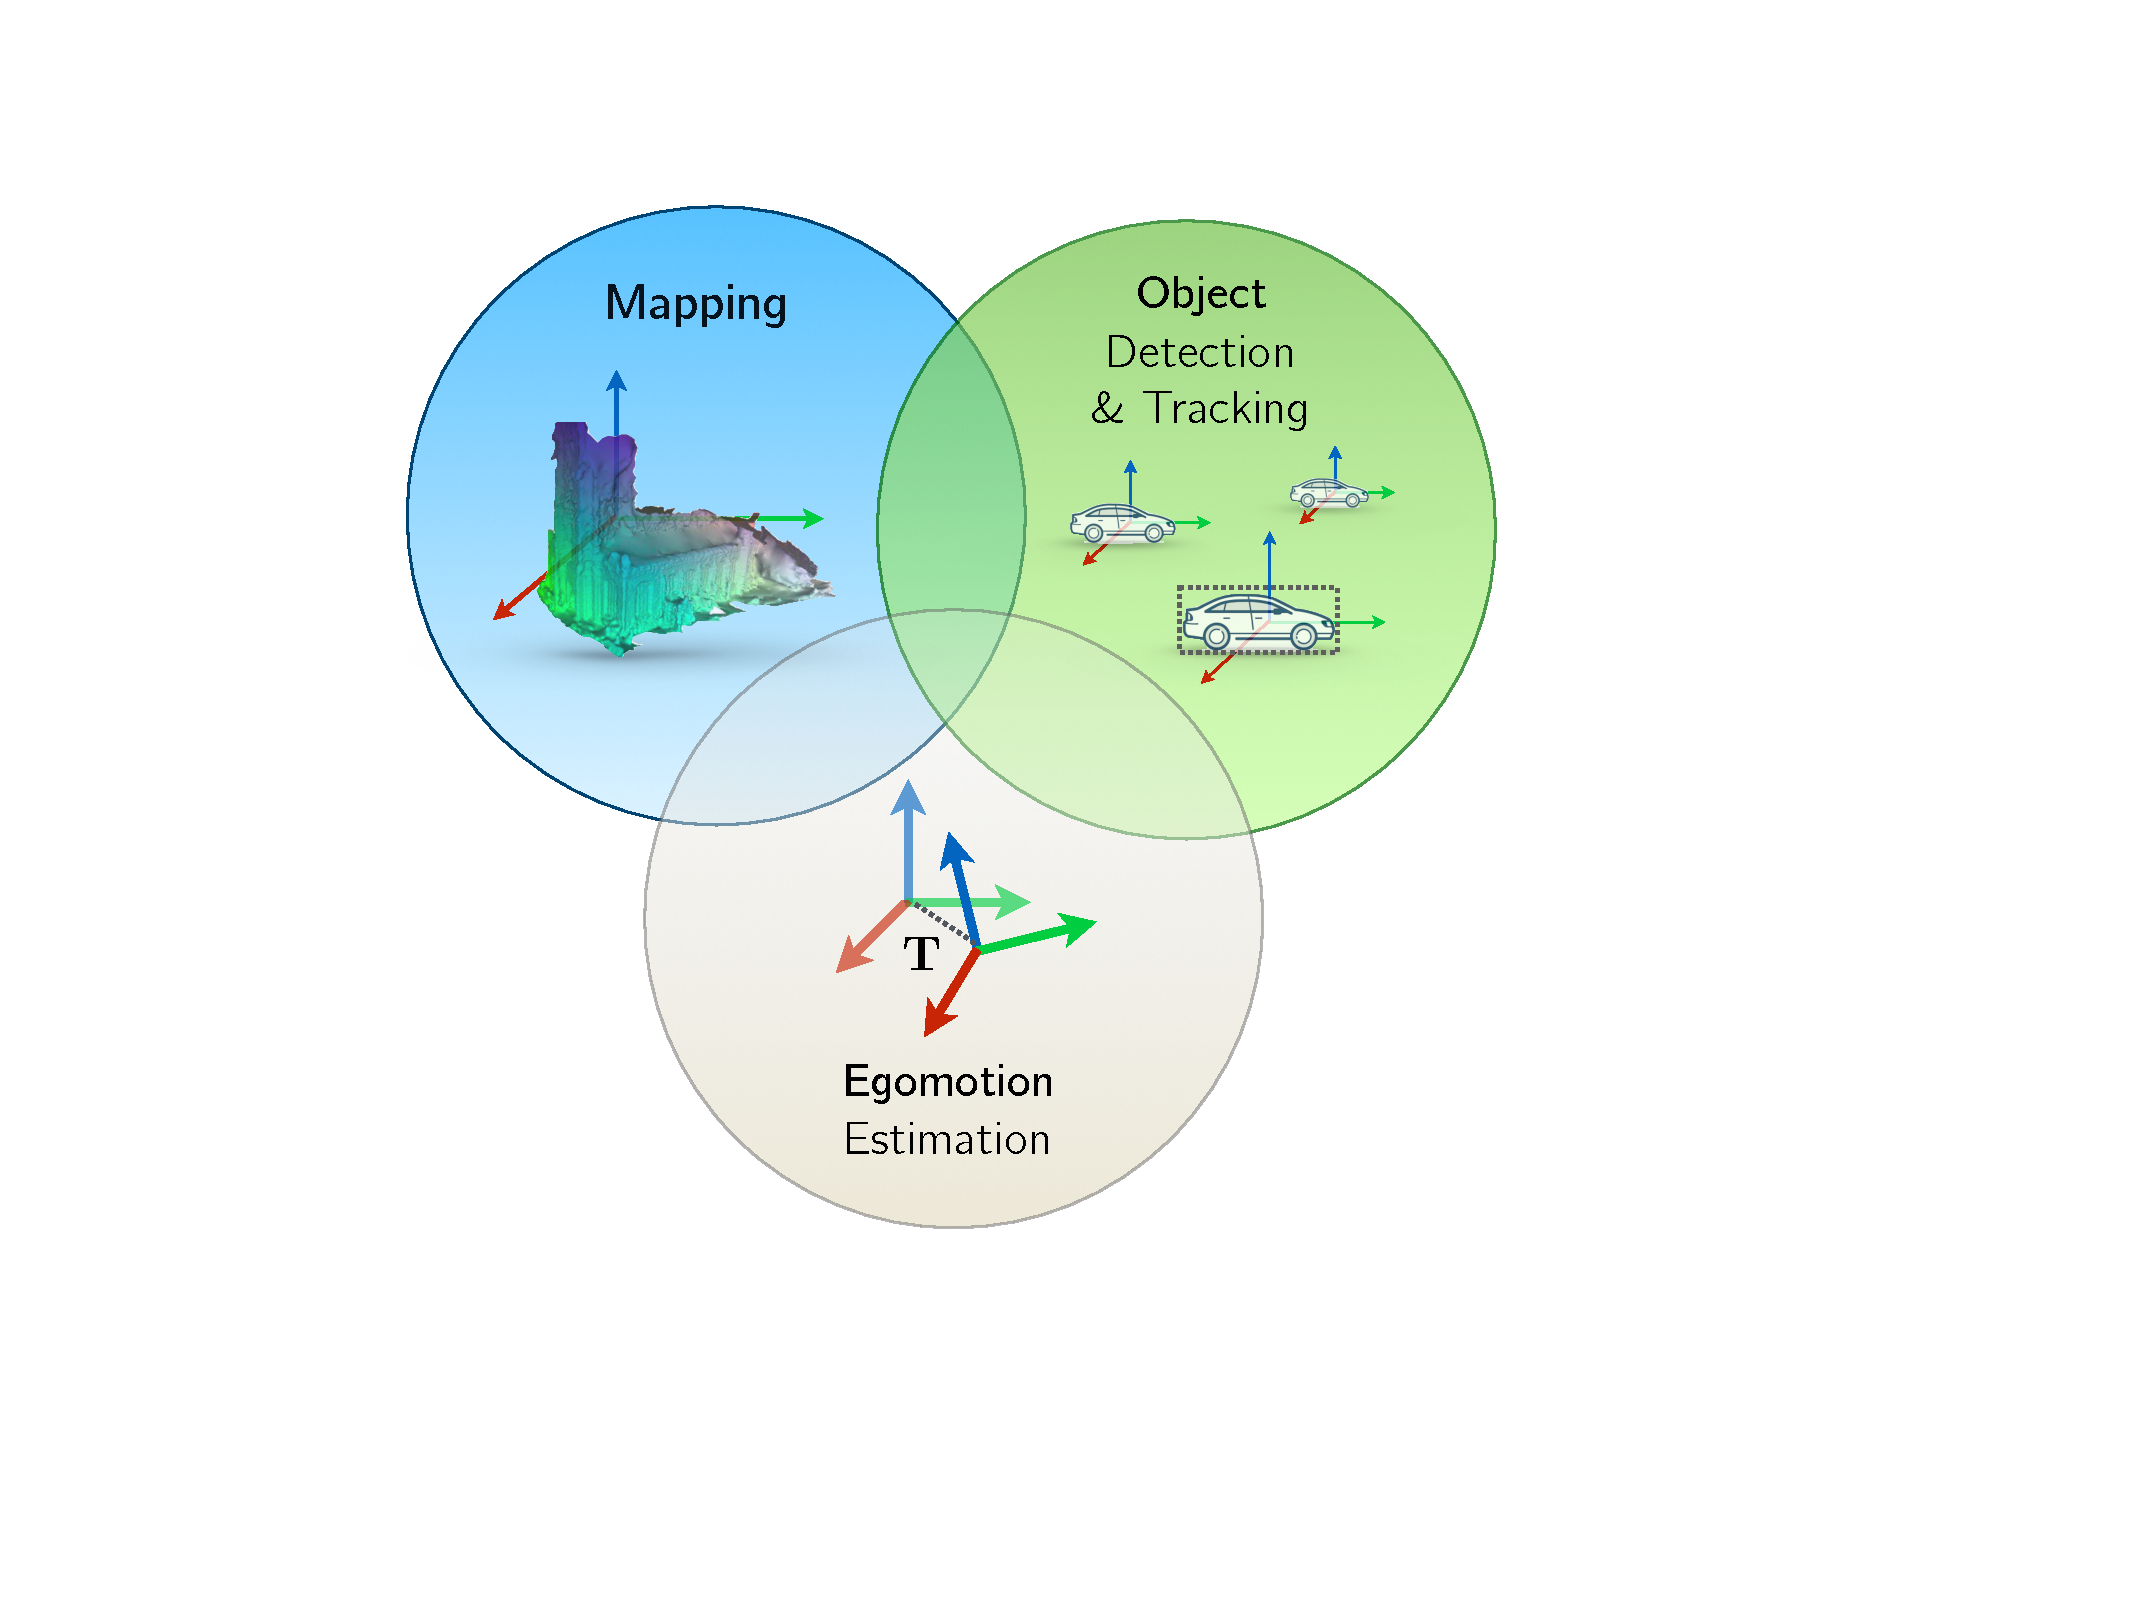
\includegraphics[width=0.45\textwidth]{introduction/venn_perception}
	\caption{Visual egomotion estimation can be useful to create maps and to detect and track other objects.}
	\vspace{1.2em}
	\label{fig:intro_state_venn}
\end{wrapfigure}

To address this, a number of researchers in the 1980s developed the technique of \textit{visual} odometry \citep{Scaramuzza2011-qr} (or VO), as a way to infer egomotion from sequentially-collected images. The mathematical basis of VO is closely tied to the technique of photogrammetric \textit{bundle adjustment} \citep{triggs_bundle_2000} which originates from 19th century photogrammetry \citep{albertz_look_2007}.



% Modern mobile autonomy was largely born out of  .
% 
%https://mars.nasa.gov/resources/22342/opportunity-legacy-pan-true-color/
\begin{figure}
  \begin{center}
    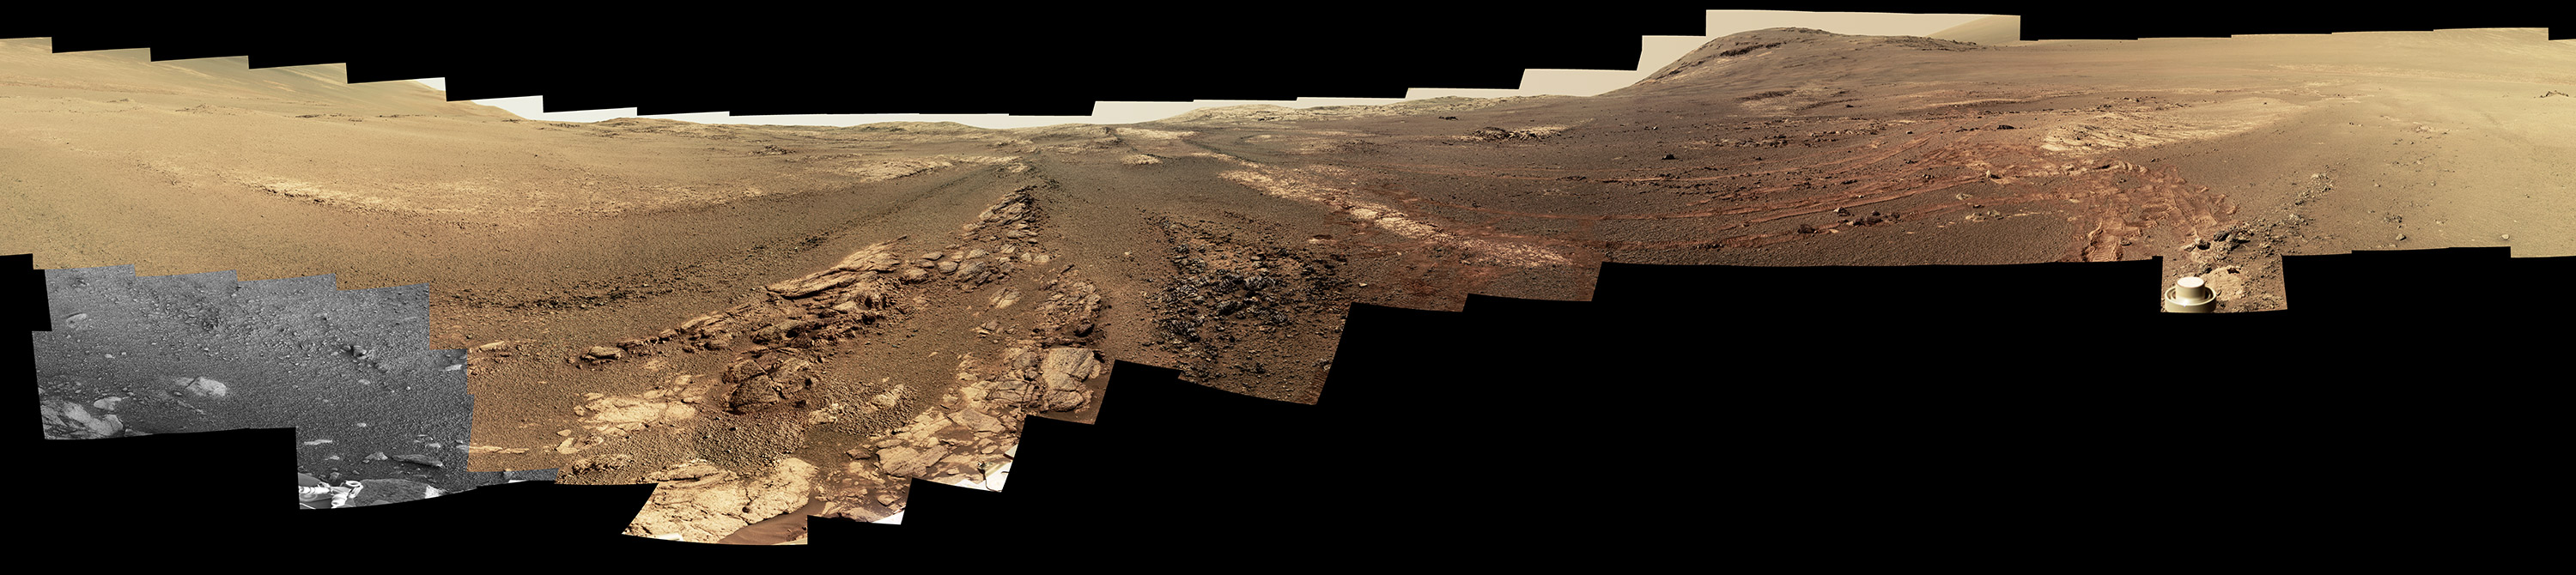
\includegraphics[width=\textwidth]{introduction/pancam-panorama-opportunity}
  \end{center}
  \caption{The last 360 degree panorama of the rocky Martian surface taken by the Pancam apparatus of the Mars Exploration Rover, \textit{Opportunity}, at its final resting place, the western rim of the Endeavour Crater (\textit{credit: NASA/JPL-Caltech/Cornell/ASU}).}
    \label{fig:intro_endeavour_crater}
\end{figure}





%\begin{figure}
%         \centering
%\def\firstcircle{(0,0) circle (2cm)}
%\def\secondcircle{(60:2.75cm) circle (2cm)}
%\def\thirdcircle{(0:2.75cm) circle (2cm)}
%\scalebox{0.75}{
%\begin{tikzpicture}
%    \begin{scope}[shift={(3cm,-5cm)}, fill]
%        \fill[green!80,opacity=0.5] \firstcircle;
%        \fill[blue,opacity=0.5] \secondcircle;
%        \fill[black,opacity=0.5] \thirdcircle;
%        \draw \firstcircle node [yshift=-1ex,xshift=-2.5ex,align=center] {C. Mapping};
%        \draw \secondcircle node [above,color=white,align=center] {A. Egomotion\\estimation};
%        \draw \thirdcircle node [yshift=-1ex,xshift=3ex,color=white,align=center] {B. Object\\tracking};
%        \draw[->] (1.2,0.8) -- (3.7,3) node[right,align=left] {State\\Estimation};
%    \end{scope}
%\end{tikzpicture}         
%}
%        \caption{Venn diagrams of modern mobile autonomy.}
%        \label{fig:intro_three_venn}
%\end{figure}


 %Add some discussion about computer science vs. robotics research
 
In the nearly four decades since the first development of VO, the proliferation of compact, relatively-inexpensive, high-resolution cameras has made vision-based sensing techniques ubiquitous in mobile autonomous applications. In addition to computing egomotion, camera data can be used to build detailed maps of an environment (which can be computed in tandem with egomotion through a technique called simultaneous localization and mapping, or SLAM \citep{Cadena2016-ds}), as well as detect, track and avoid other objects (\Cref{fig:intro_state_venn}). 

\section{A Visual \textit{Pipeline}}

\begin{figure}
\begin{center}
		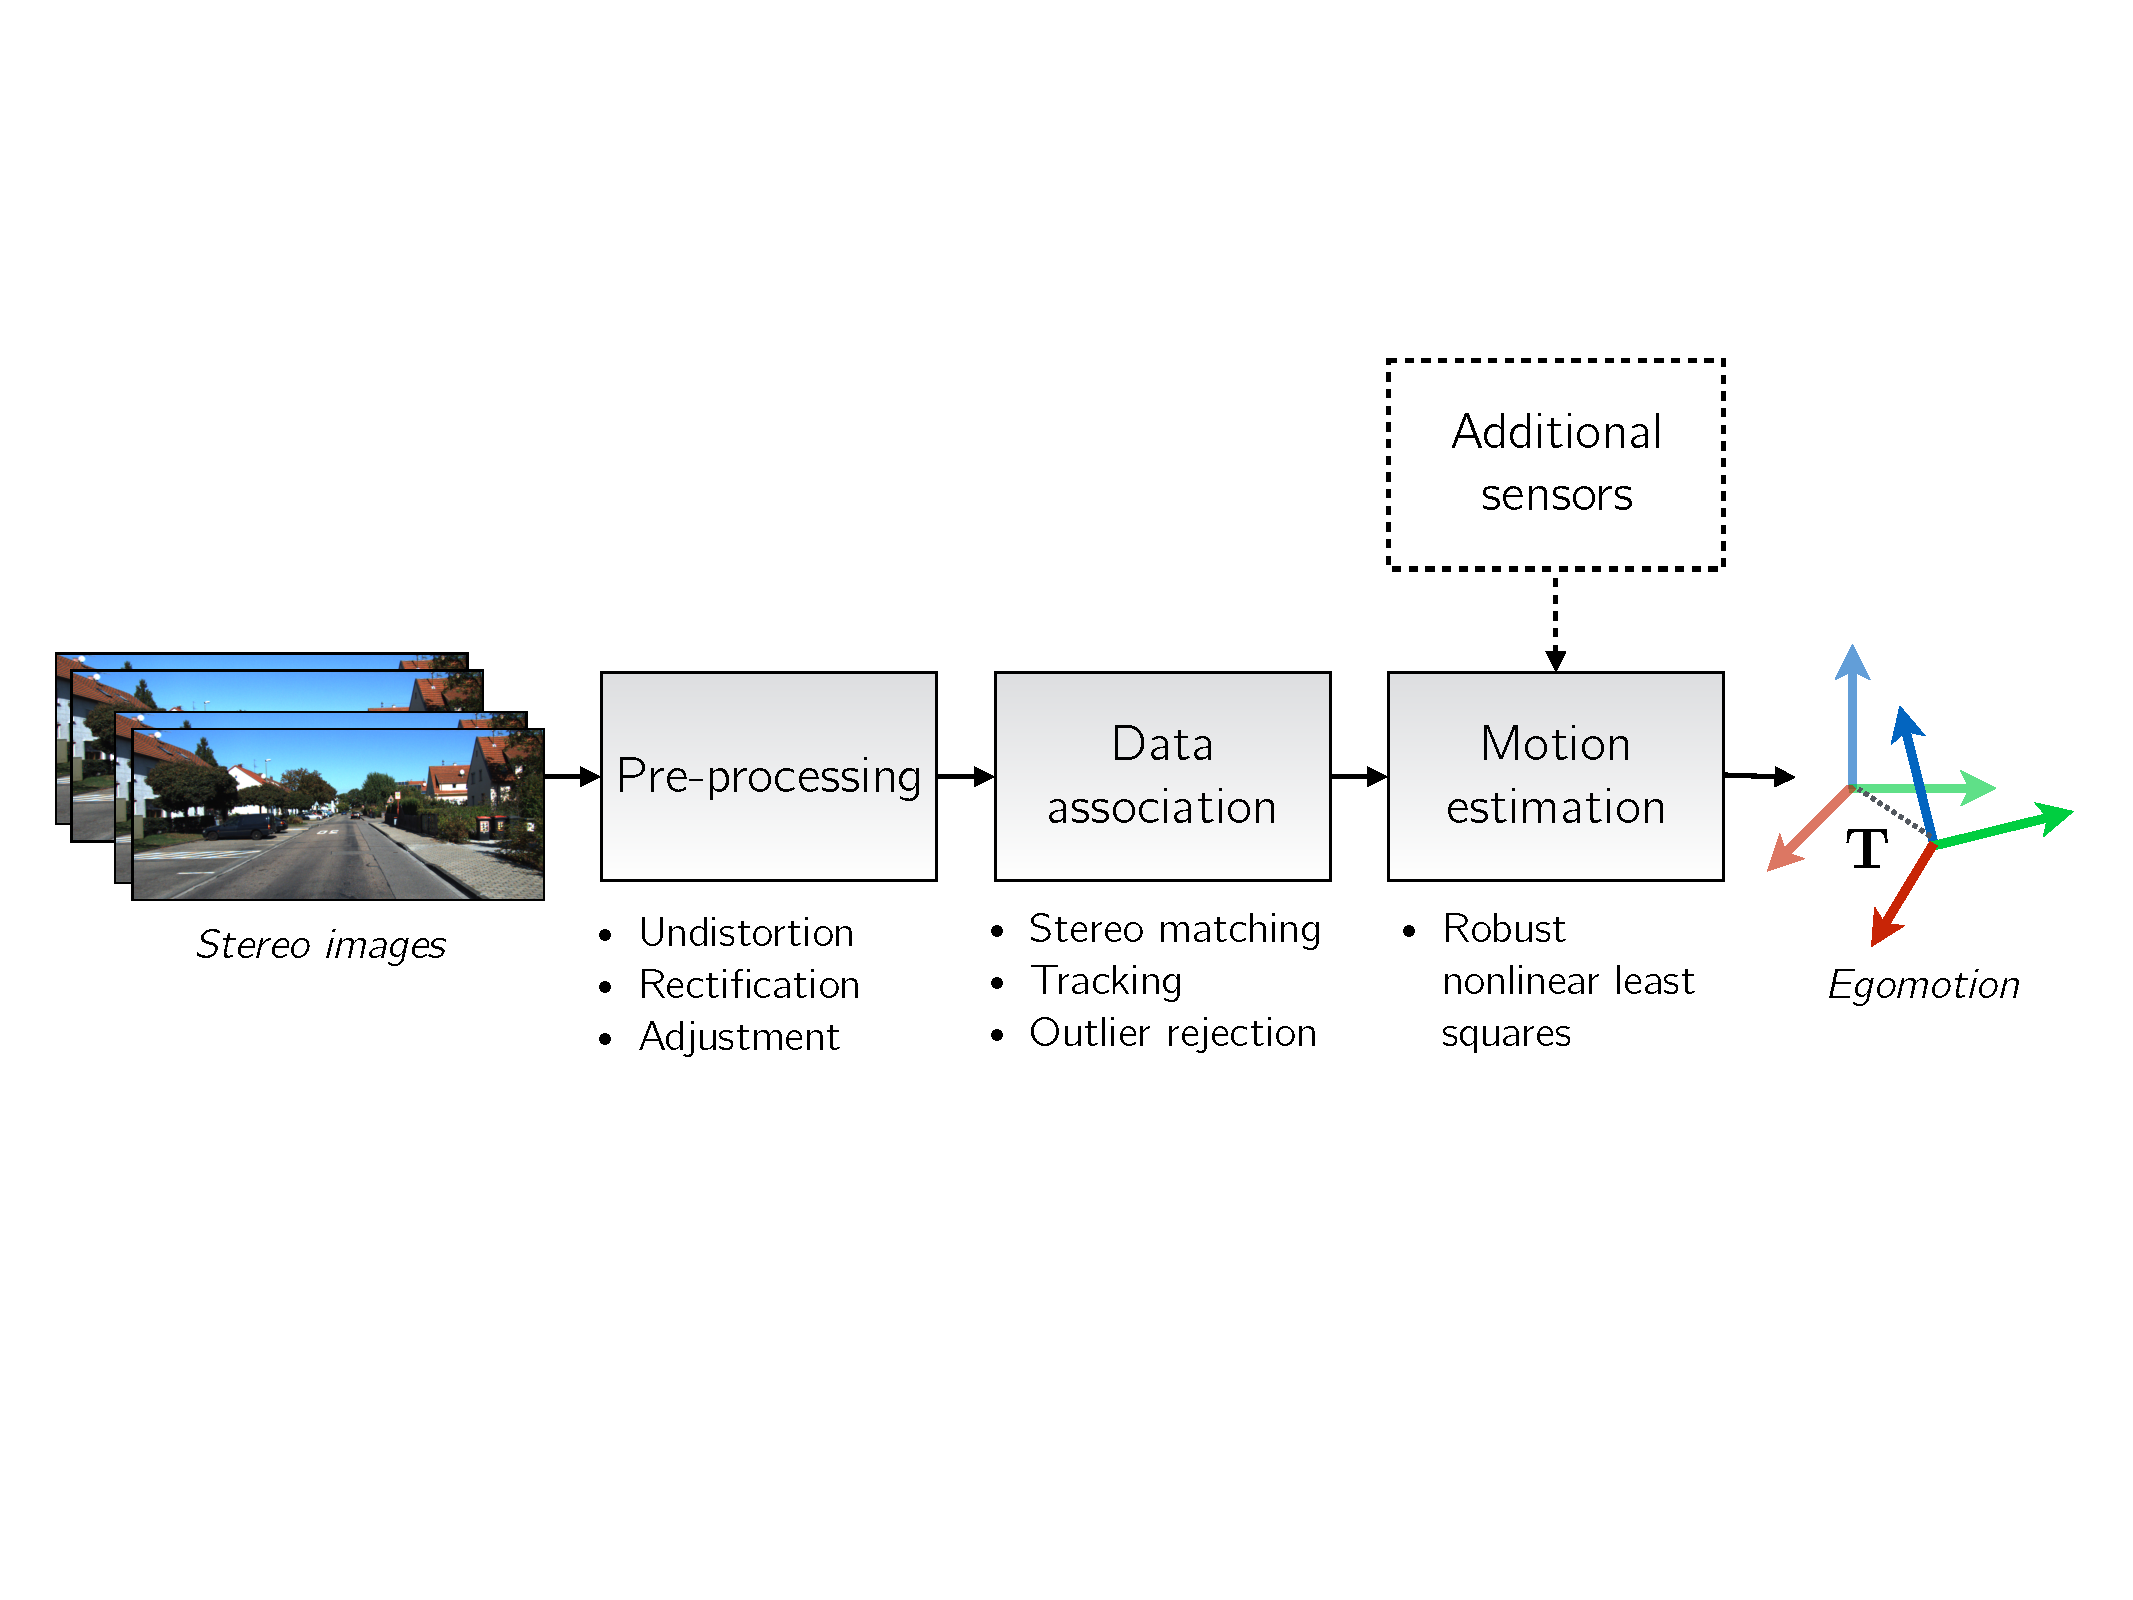
\includegraphics[width=0.98\textwidth]{introduction/vo_pipeline.pdf}
		\caption{A `classical' visual odometry pipeline consists of several distinct components with interpretable inputs and outputs. We list common examples of each component. }
  	\label{fig:intro_vo_pipeline}
\end{center}
\end{figure}


Central to \textit{classical} visual odometry algorithms (which, in this context, refers to the bulk of VO research published during what \cite{Cadena2016-ds} call the \textit{classical} and \textit{algorithmic-analysis} ages of VO and SLAM research between 1986 and 2015) is the idea of a processing pipeline. A  pipeline consists of several connected computational `blocks' or 'stages' that have interpretable inputs and outputs.  By carefully processing information contained within raw sensor data, pipelines facilitate the construction of complex state estimation architectures that can fuse visual observations with other sensors of varied modality to create maps and models of the external world and infer the egomotion of a mobile platform within it. In this dissertation, we will largely deal with the improvement of a canonical visual odometry pipeline-- we illustrate its major components in \Cref{fig:intro_vo_pipeline}. 

Broadly, VO solutions based on the idea of hand-crafted pipelines \citep{Leutenegger2015-fk, Cvisic2015-mt, Tsotsos2015, Alcantarilla2016-kv, forster2014svo, wang_stereo_2017, engel_direct_2018} have achieved impressive localization accuracy within a variety of settings. They have been used to compute the egomotion of self-driving cars through urban roads, and track autonomous drones through aggressive flying maneuvers. 

Building on momentum from the computer vision community, a significant part of the visual state estimation literature has also considered replacing classical pipelines with parametric modelling through deep convolutional neural networks (CNNs) and data-driven learning. Although initially developed for image classification \citep{LeCun2015-qf}, CNN-based measurement models have been applied to numerous problems in visual state estimation including homography estimation \citep{DeTone2016-ue}, single image depth reconstruction \citep{Garg2016-ip},  camera re-localization \citep{Kendall2016-zf}, and place recognition \citep{Sunderhauf2015-is}. A number of recent CNN-based approaches have also tackled the problem of visual egomotion estimation, often purporting to obviate the need for classical visual localization pipelines by learning pose changes \textit{end-to-end}, without requiring intermediate outputs \citep{Melekhov2017-dl, Handa2016-hm, Oliveira2017-lt}.

In light of these new approaches, debate has emerged within the robotics and computer vision communities regarding the extent to which data-driven parametric models should replace pipelines. Although classical approaches can achieve high accuracy under nominal conditions, deep data-driven networks have the potential to improve upon them in two respects.

First, owing to their representational power, deep parametric networks have the potential to learn bespoke data associations that are robust to (1) large viewpoint changes, (2) moving objects, and (3) self-similar visual textures (e.g., indoor walls, grass, sky, etc.). Such robust, invariant data associations have been the holy-grail of hand-crafted pipelines, and traditional data association methods must be carefully tuned to work well in a given setting \citep{schonberger_comparative_2017}.

Second, deep parametric regression of egomotion has the potential to more efficiently use dense high-dimensional visual data. To remain computationally tractable, classical VO pipelines typically take one of two approaches.  First, some pipelines \citep{Leutenegger2015-fk,Cvisic2015-mt} choose to indirectly summarize visual data by extracting and matching a set of sparsely-distributed salient \textit{features}. These features may be robust to some of the effects mentioned above, but, by construction, they discard large portions of visual data that may inform more accurate egomotion estimates. Alternatively, other methods \citep{forster2014svo, wang_stereo_2017,  engel_direct_2018} may instead choose to match photometric intensity directly through an assumption of photometric consistency. This relatively simple schema permits dense data association but can be a poor assumption in the presence of large viewpoint changes or non-Lambertian surfaces. Further, this approach yields a high number of data associations and produces a highly non-convex objective that requires care to optimize. 

In contrast, deep networks built on basic image operations with modern computationally-efficient implementations have the potential to avoid the pitfalls of both of these approaches while remaining tractable (assuming appropriate hardware). Despite this potential, current end-to-end learning techniques for egomotion estimation have a number of disadvantages (see \Cref{tab:intro_classical_vs_deep}). They often generalize poorly to new environments, come with few analytical guarantees, provide only point estimates of latent parameters, and do not allow for intermediate representations that have been shown to improve generalization performance on visual tasks \citep{Zhou2019-se}. Indeed, according to one benchmark, the most accurate visual egomotion approach at the time of writing\footnote{Based on the KITTI Odometry benchmark leaderboard at \url{http://www.cvlibs.net/datasets/kitti/eval_odometry.php}.} remains a classical pipeline based on carefully selected sparse features.

\begin{figure}
\begin{center}
		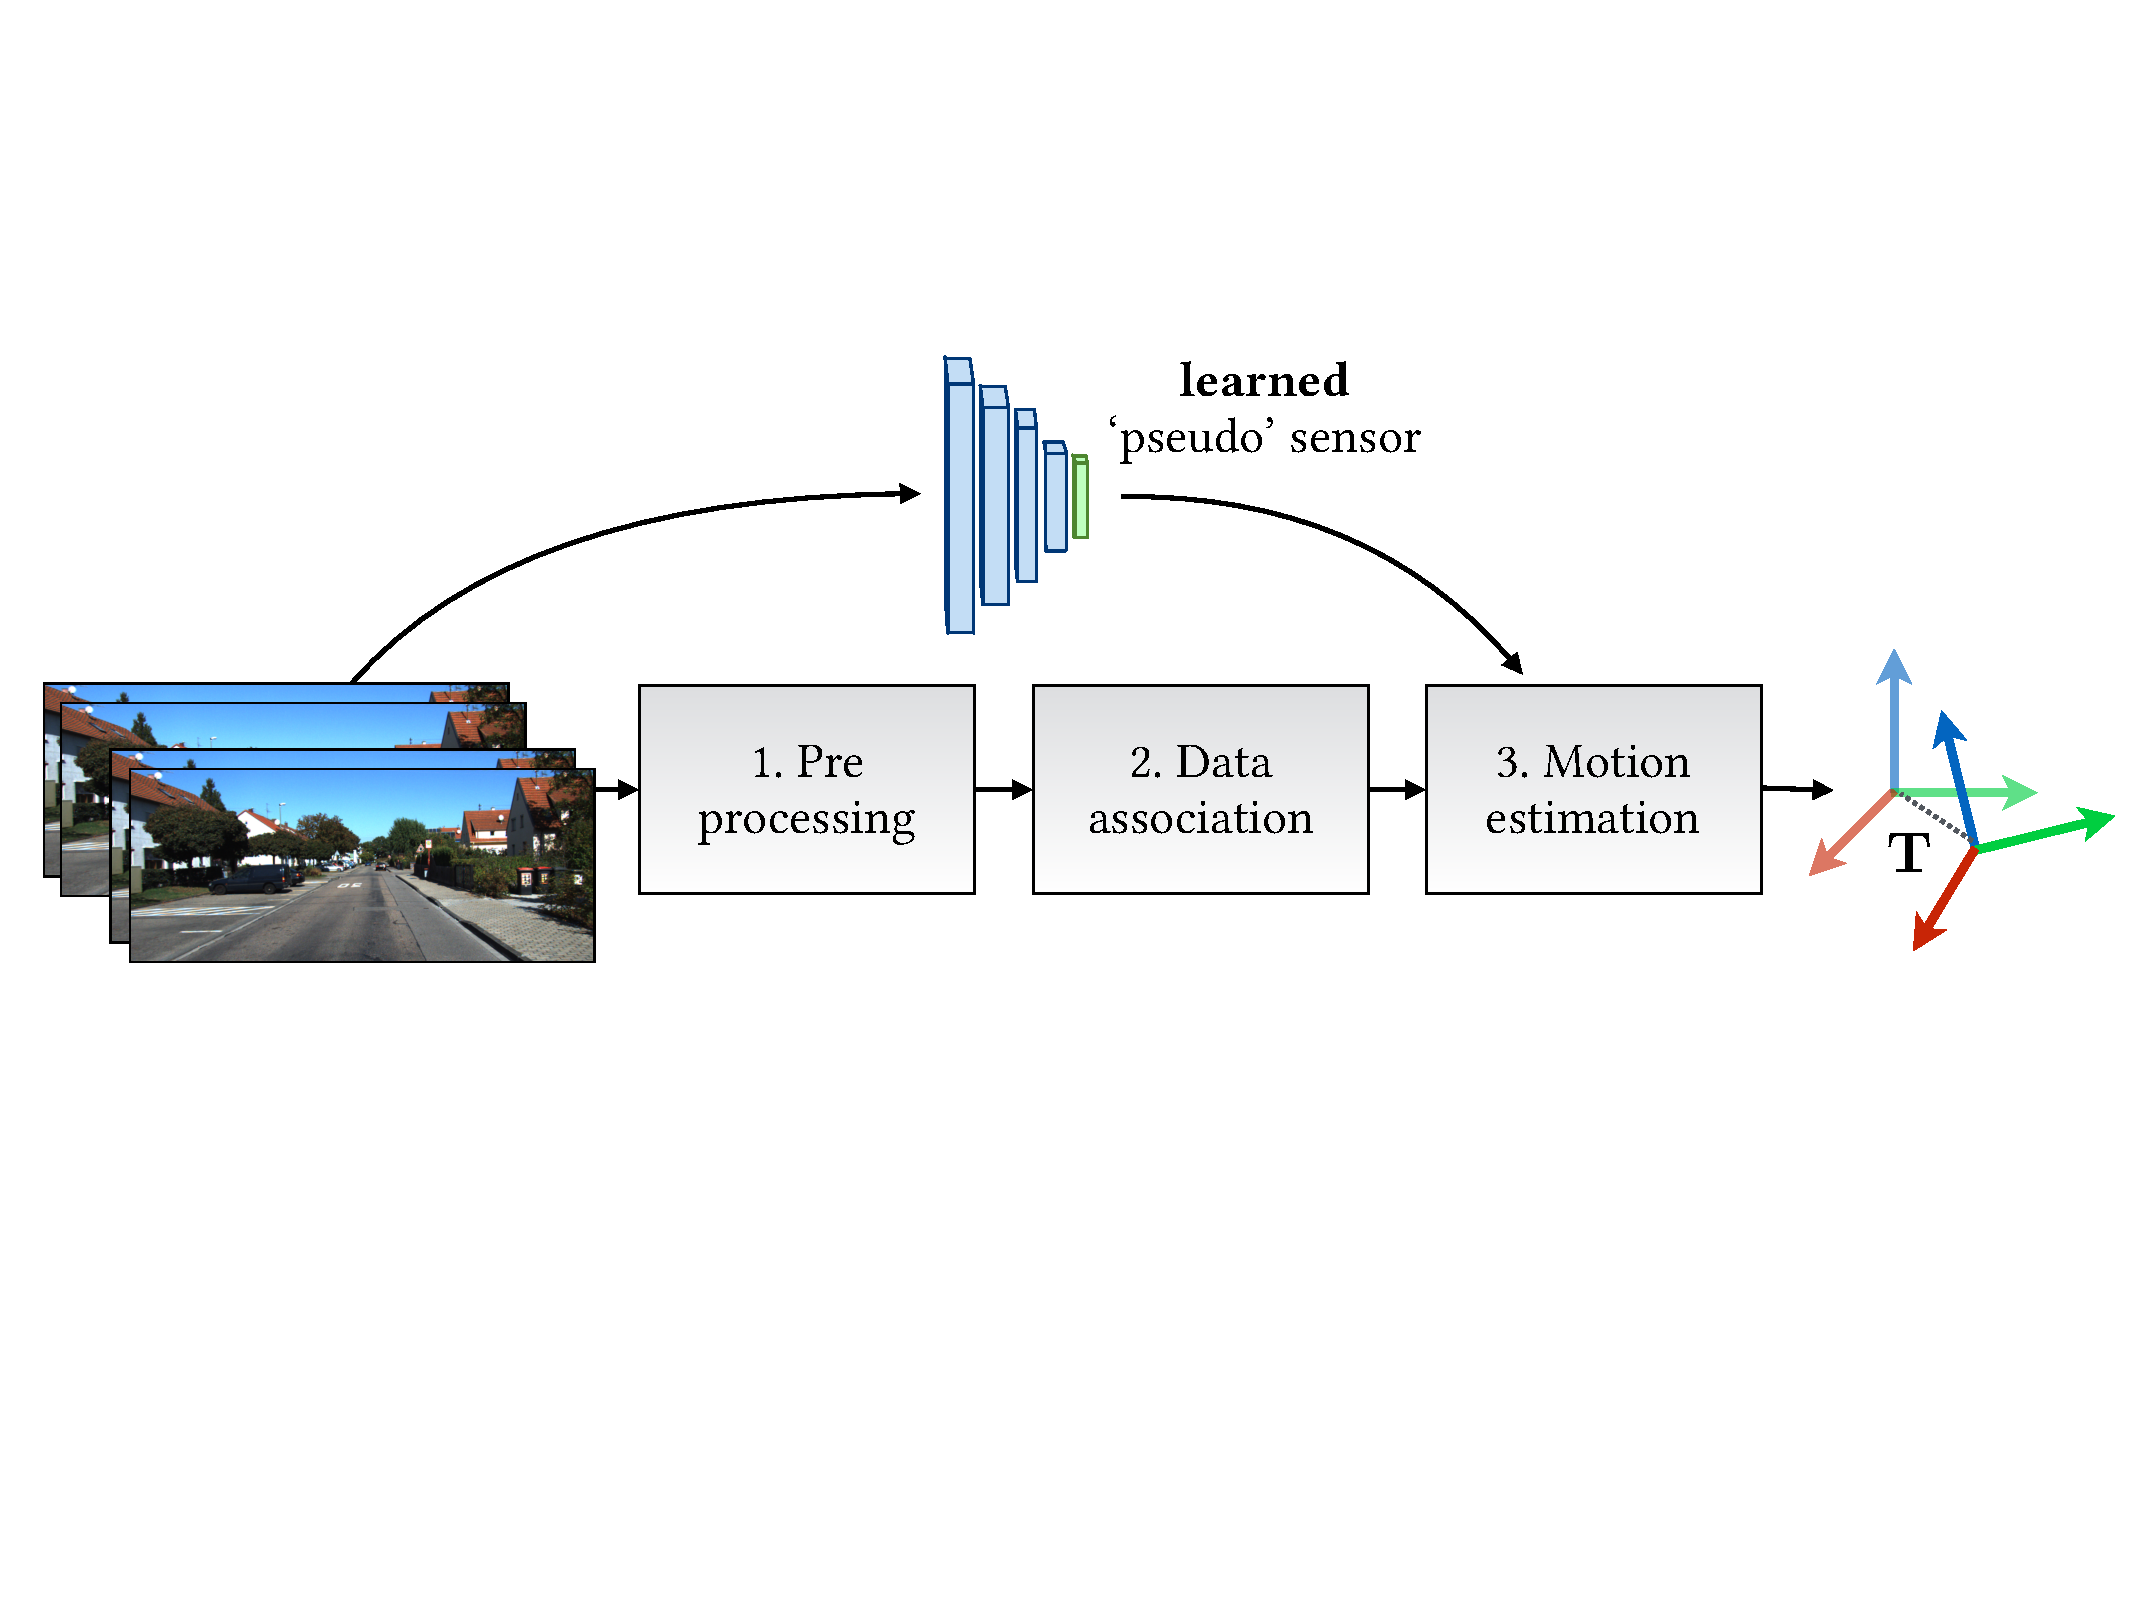
\includegraphics[width=0.98\textwidth]{introduction/pseudo_sensor.pdf}
		\caption{A learned \textit{pseudo-sensor} extracts latent information from the same data stream.}
  	\label{fig:intro_pseudo_sensor}
\end{center}
\end{figure}


\begin{table}[h!]
	\caption{A comaprison of pipelines and end-to-end deep models for visual egomotion estimation.}
	\begin{threeparttable}
	\begin{tabular}{m{0.18\textwidth}m{0.38\textwidth}m{0.38\textwidth}}
		\toprule
		& \textbf{Classical Pipelines} & \textbf{Deep Models} \\ \midrule  
		\textit{Maturity} & Decades of literature \& domain knowledge & Nascent with few uses in mobile autonomy \\
		& & \\
		\textit{Interpretability} & Good, each component has interpretable input and output & Poor, often with no interpretable intermediate outputs \\
		& & \\
		\textit{Uncertainty} & Foundational to \textit{probabilistic robotics} & Few nascent methods (Monte-carlo Dropout \citep{Gal2016-ny}, Bootstrap \citep{Osband2016})  \\
		& & \\
		\textit{Robustness} & Empirically generalizable \citep{Zhou2019-se} & Highly dependant on training data\\
		& & \\
		\textit{Flexibility} & Limited by ingenuity of designer & Limited by training data \\
		\bottomrule
	\end{tabular}
\end{threeparttable}
\label{tab:intro_classical_vs_deep}
\end{table}

\section{The Pseudo-Sensor}

As mobile autonomy enters the robust-perception age \citep{Cadena2016-ds}, classical pipelines that work in limited contexts will need to be adapted and augmented to ensure they can operate over longer time periods, and through challenging environments. However, replacing these performant pipelines completely with learned approaches, is in our view, unnecessary. Instead, we propose the paradigm of the  \textit{pseudo-sensor} (\Cref{fig:intro_pseudo_sensor}). A \textit{pseudo-sensor} is a machine-learning-based (hyper-)parametric model that extracts latent information from existing sensor data that is difficult to model analytically. Pseudo-sensors leverage the representational power of modern data-driven learning techniques to extract useful quantities that make existing classical pipelines more consistent and accurate in a given environment. In this dissertation, we present four such pseudo-sensors. In each case, the output of the pseudo-sensor is fused with a classical visual odometry pipeline to produce better motion estimates. To accomplish this fusion, we rely on two approaches. The first (Predictive Robust Estimation, or PROBE, \Cref{ch:probe}), uses the paradigm of a pseudo-sensor to infer a heteroscedastic noise model based on sensor data. By predicting uncertainty information, PROBE effectively re-scales a robust loss function to better account for deleterious visual effects. The second approach (used by Sun-BCNN, DPC-Net, and HydraNet,  \Cref{ch:sun-bcnn,ch:dpc,ch:hydranet} respectively) produces geometric quantities (probabilistic estimates of an illumination source, $\LieGroupSE{3}$ corrections to existing egomotion estimates, and independent probabilistic rotation estimates, respectively), that can be fused with the original egomotion estimate through pose graph optimization.

%\section{Outstanding Issues in the Field}

%\subsection{The limits of homoscedastic noise models}
%
%Although several state-of-the-art state estimation pipelines  \citep{Leutenegger2015-fk, Cvisic2015-mt} leave observation uncertainty associated with sensor measurements as a static tuning parameter, recent work \citep{Vega-Brown2014-sb, Hu2015-uw} suggests that using a stationary, homoscedastic noise in observation models can often reduce the consistency and accuracy of state estimates. This is especially true for complex, inferred measurement models. In foot-mounted navigation, the inferred zero velocity detector may be more or less informative depending on the exact type of motion and individual gait. In visual data, inferred visual observations can be degraded not only due to sensor imperfections (e.g. poor intrinsic calibration, digitization effects, motion blur), but also as a result of the observed environment (e.g. self-similar scenes, specular surfaces, textureless environments). Indeed, robust costs \cite{Alcantarilla2016-kv, MacTavish2015-wt, Agarwal2013-jq} and whiteness tests \citep{Tsotsos2015} have commonly been used to alleviate the problem of poor noise modelling, but more work is required to better learn uncertainty in complex measurement models.
%
%
%\subsection{Deep, learned models with no uncertainty estimates}
%
%Although the paradigm of deep neural networks has resulted in several significant achievements in the fields of computer vision \citep{LeCun2015-qf}, these types of models have largely focused on point estimates (in either regression or classification) without any principled uncertainty estimates. Recently, the regularization techniques of dropout and dropconnect in Convolutional Neural Networks have been linked with approximate variational inference in homoscedastic Gaussian Processes \citep{Gal2015-bf, Kendall2016-zf, McClure2016-ai}, and the statistical technique of \textit{bootstrapping} has been applied to Deep Q Networks \citep{Osband2016-jg} to infer uncertainty, but both techniques are in their infancy. Recent work \citep{Osband_undated-wl} has also suggested that the former technique of dropout-based `uncertainty' is actually a measure of \textit{risk} (i.e., stochasticity in the measurements) and not \textit{uncertainty} over state parameters. Further, the same work showed that even this risk quantification can be arbitrarily bad given a fixed dropout parameter (which is typically the case).
%
%\subsection{Integration of deep models into state estimation pipelines}
%
% To integrate the power of deep networks into state estimation algorithms, the recent literature differs in how to proceed. While some attempt to parametrize geometric transformations in their unconstrained state, and then learn the resulting state within a deep network regression optimization \citep{Costante2016-hb, Kendall2015-kh}, others integrate deep networks within outer estimation loops \citep{Haarnoja2016-ph}. Yet other work has used the neural network as an error correcting mechanism on top on an existing kinematic or dynamic model \citep{Punjani2015-pj}. This integration is made more difficult by the lack of uncertainty estimates associated with many learned measurement models in the computer vision and machine learning literature.
% 
 
\section{Original Contributions}

\begin{figure}[h!]
\begin{center}
		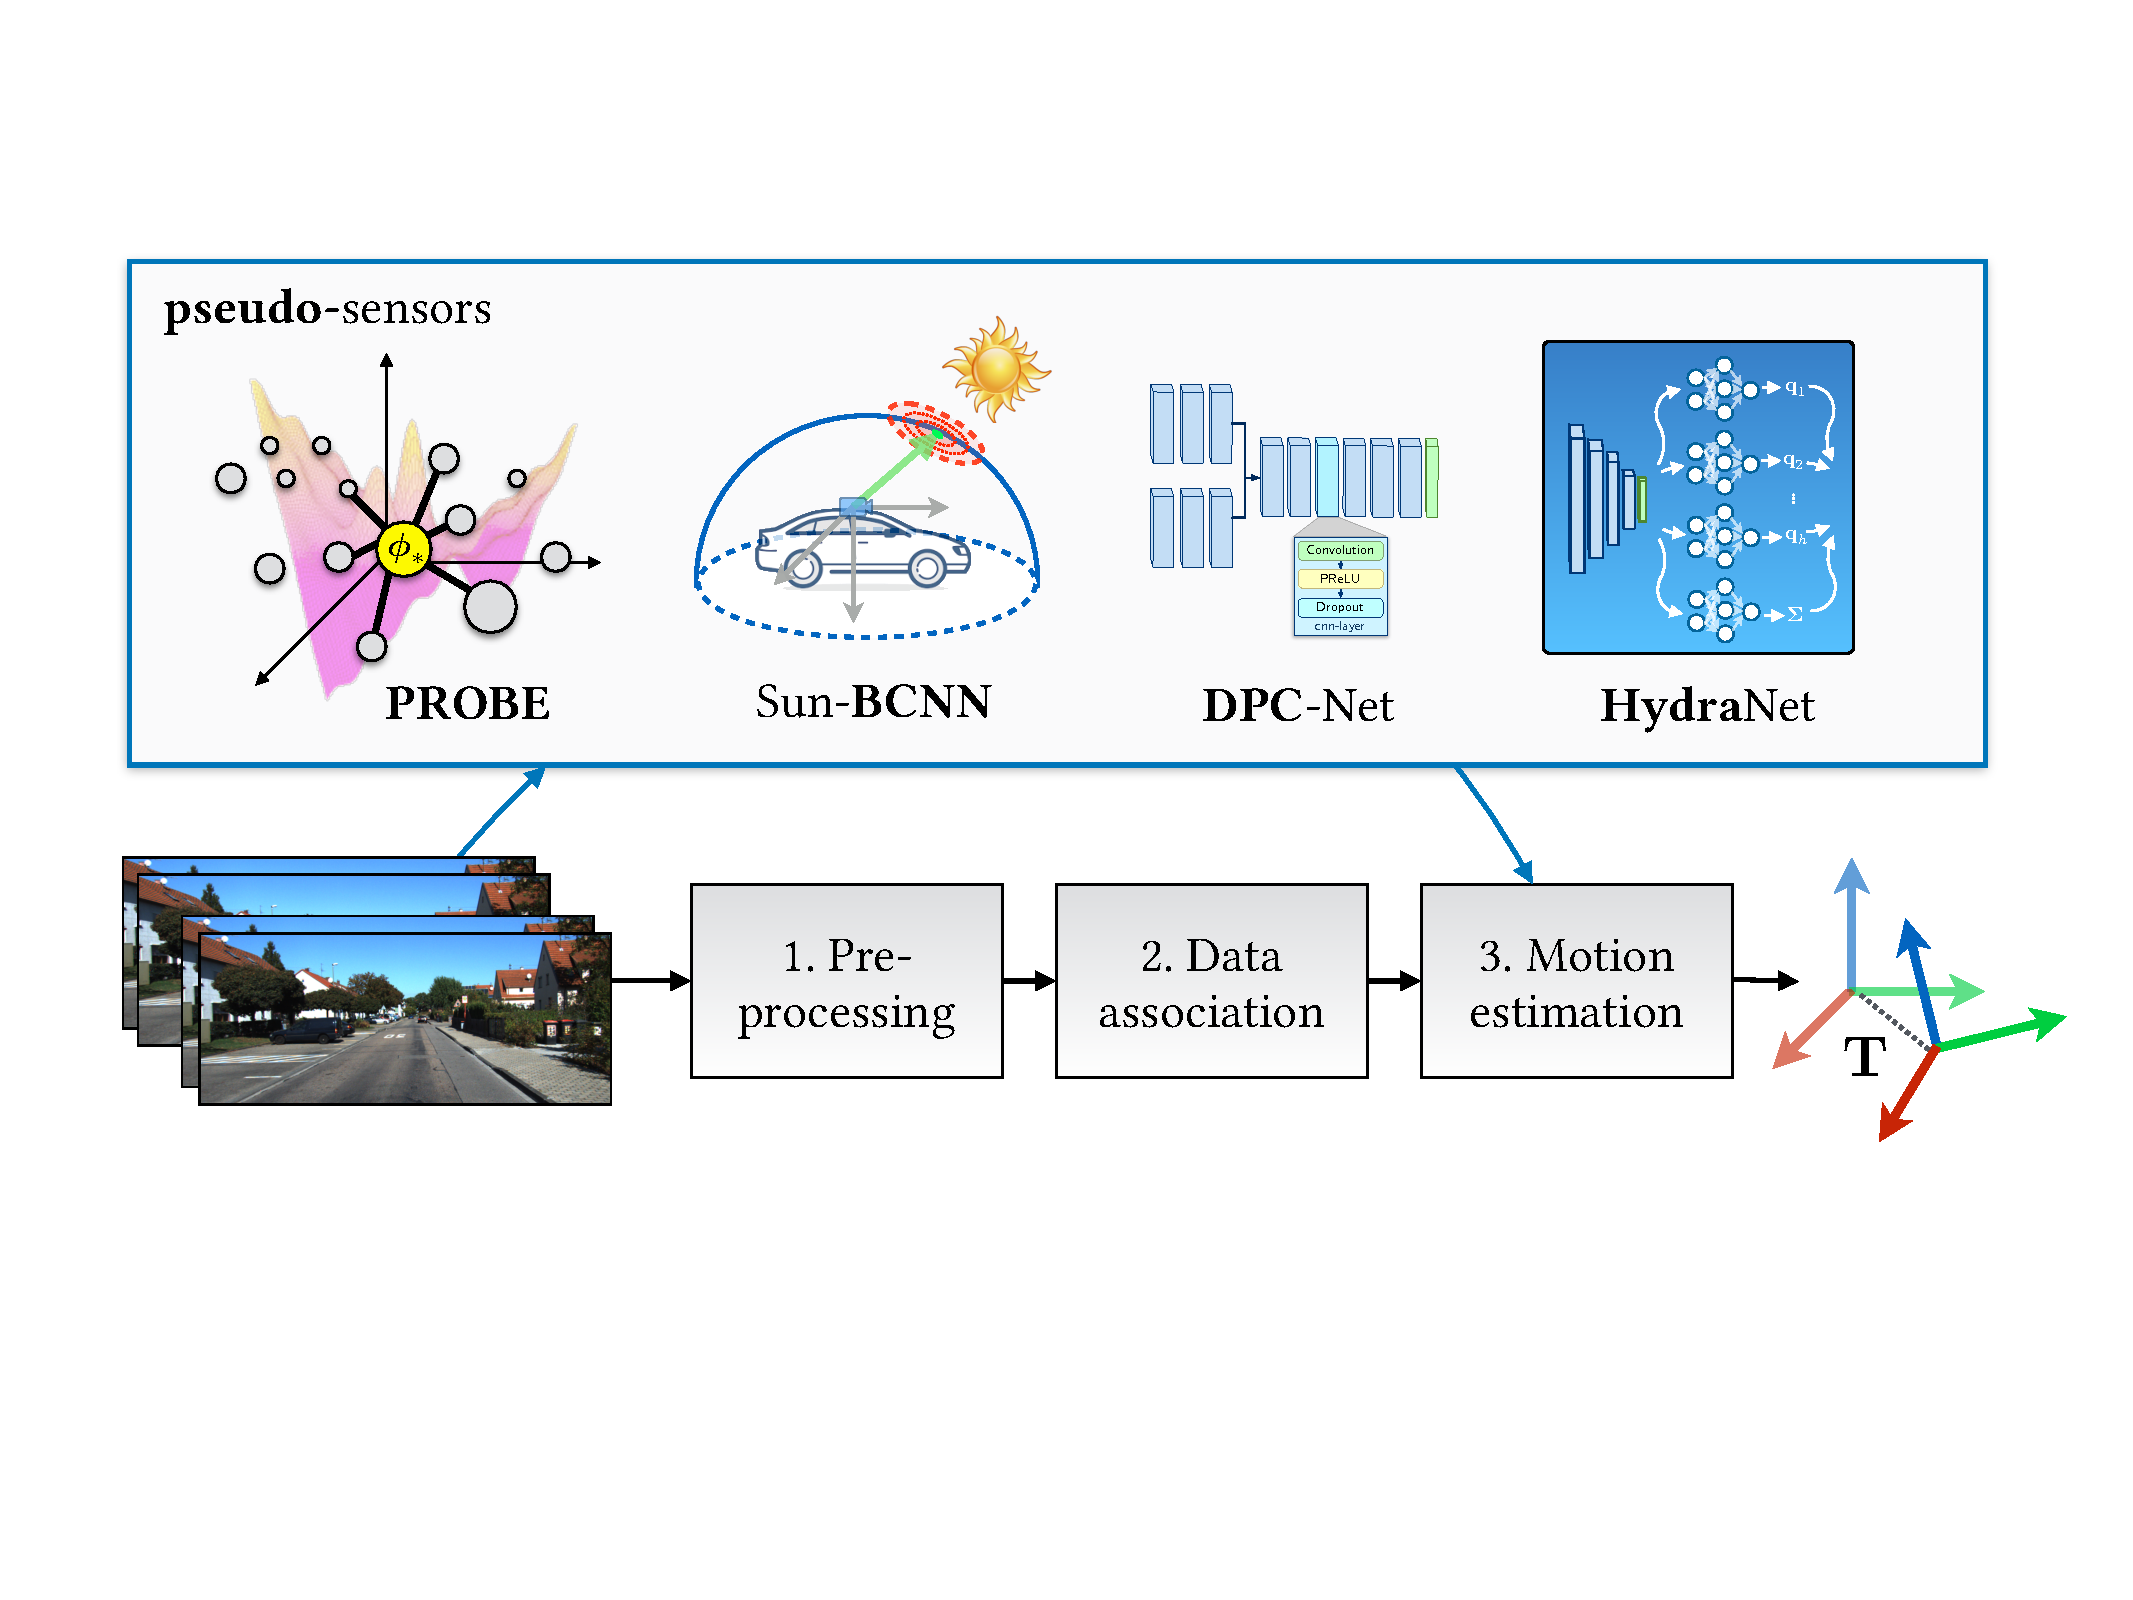
\includegraphics[width=0.98\textwidth]{introduction/all_pseudo_sensors.pdf}
		\caption{Four \textit{pseudo-sensors} that improve 'classical` egomotion estimation through data-driven learning.}
  	\label{fig:intro_pseudo_sensors}
\end{center}
\end{figure}


This dissertation consists of several published contributions under the umbrella of \textit{learned pseudo-sensors} that improve a canonical visual egomotion pipeline. Before detailing each pseudo-sensor, we present some mathematical foundations (\Cref{ch:math}) and a common baseline for a feature-based stereo visual odometry pipeline (\Cref{ch:vo}) which all four methods build upon. In total, there are two journal papers and five conference papers associated with our work. Below, we briefly summarize each of the pseudo-sensors and list the publications that are associated with each.
\begin{enumerate}
\item \textbf{PROBE: Predictive Robust Estimation},  \\
Predictive Robust Estimation (\Cref{ch:probe}, Appendix \ref{app:appendix_probe_knn}) builds a predictive model for observation uncertainty from training data. To do this, we collaborate with William Vega-Brown at MIT to adapt the technique of Generalized Kernel (GK) estimation \citep{Vega-Brown2014-sb} to visual odometry. Generalized Kernel estimation allows us to build an efficient Bayesian model for stereo tracking uncertainty. By setting a prior on covariance, we derive a `robust' objective that can be \textit{predictively} scaled to improve the accuracy and consistency of a feature-based stereo visual odometry pipeline. PROBE is associated with three publications: \cite{2015_Peretroukhin_PROBE,2015_Peretroukhin_Get,Peretroukhin2016-om}. The first two publications explore useful predictors for uncertainty and build a non-Bayesian isotropic covariance model. The latter publication presents the Bayesian GK approach.
%\begin{itemize}
%\item \bibentry{2015_Peretroukhin_PROBE},
%\item \bibentry{2015_Peretroukhin_Get},
%\item \bibentry{Peretroukhin2016-om}.
%\end{itemize}

\item \textbf{Sun-BCNN: Learned Probabilistic Sun Sensor} \\ 
Sun-BCNN (\Cref{ch:sun-bcnn}) is a virtual sun sensor based on a Bayesian Convolutional Neural Network (BCNN) that was developed in collaboration with Lee Clement. Much like a dedicated hardware sun sensor, Sun-BCNN infers a probabilistic estimate of the direction of the sun that can be used to inject orientation information into an egomotion pipeline. However, unlike dedicated sensors, Sun-BCNN requires no additional hardware and can predict both a mean and uncertainty from a single RGB image. It is associated with three publications: \cite{2017_Clement_Improving,2017_Peretroukhin_Reducing,2018_Peretroukhin_Inferring}. The first publication consists of initial exploratory work on virtual sun sensors, while the second presents the BCNN formulation. The final publication is an extended journal article that summarizes the results of the prior two conference publications and adds two novel contributions: (1) further experimental validation on visual data collected in the Canadian High Arctic and around Oxford, UK, and (2) investigations into the effect of cloud cover and the possibility of generalization across datasets. 


\item \textbf{DPC-Net: Learned Pose Corrections} \\
Deep Pose Correction (\Cref{ch:dpc}) is an approach to improving egomotion estimates through $\LieGroupSE{3}$ pose corrections learned with deep networks. As part of this work, we derive a novel loss function based on Lie theory that permits the learning six degree-of-freedom pose residuals in a supervised learning framework. After training, our Deep Pose Correction Network (DPC-Net) predicts low-rate, `small' \textit{corrections} that can be fused with egomotion estimates from a canonical pipeline. DPC-Net does not require any modification to an exisiting pipeline, and can learn to correct multi-faceted errors from estimator bias, sensor mis-calibration or environmental effects. It is associated with one journal publication, \cite{2018_Peretroukhin_Deep}.

\item \textbf{HydraNet: Learned Probabilistic Rotation Estimation}

Finally, HydraNet (\Cref{ch:hydranet}) is a multi-headed network structure that can regress probabilistic estimates of rotation (elements of the matrix Lie group, $\LieGroupSO{3}$) that account for both aleatoric and epistemic uncertainty. HydraNet builds upon results from both Sun-BCNN and DPC that show that correcting rotation is critical to accurate egomotion estimation.  Towards this end, HydraNet is designed to produce well-calibrated notions of uncertainty over $\LieGroupSO{3}$  that facilitate fusion with classical egomotion pipelines through a probabilistic factor graph formulation. It is associated with the publication, \cite{2019_Peretroukhin_Deep}.

\end{enumerate}

%\subsection{Software Contributions}
%
%\begin{itemize}
%\item DPC-Net
%\item SO(3) Learning
%\item \texttt{liegroups}
%\item pyslam 	
%\end{itemize}






